\section{Разработка библиотеки линейной алгебры на GPGPU}

Разработка библиотеки \textit{Cubool}~\cite{net:cubool_project}, предоставляющей примитивы линейной булевой алгебры для работы с разреженными данными, осуществляется в рамках исследовательского проекта лаборатории языковых инструментов JetBrains Research.

\subsection{Примитивы и операции}

Основным примитивом библиотеки является разреженная матрица булевых значений, которая хранится в видеопамяти видеокарты в формате \textit{CSR} (compressed sparse row), который позволяет использовать $O(V + E)$ памяти для хранения матрицы смежности графа. Существуют и другие форматы хранения разреженных матриц: \textit{CSC} (compressed sparse column), \textit{COO} (coordinate list) и так далее. Однако CSR формат был выбран на основе результатов работы~\cite{inproceedings:spgemm_mem_saving_for_nvidia}, так как он позволяет эффективно реализовать операцию матричного умножения в условиях ограниченного объема доступной видеопамяти. 

В качестве поэлементных операций сложения и умножения используются \textit{логическое-или} и \textit{логическое-и}. Основные функции работы с матрицами для реализации алгоритмов~\cite{inproceedings:matrix_cfpq, inbook:kronecker_cfpq_adbis} представлены ниже:

\begin{itemize}
    \item Создание матрицы $M$ размера $m \times n$
    \item Удаление матрицы $M$ и освобождение занятых ею ресурсов
    \item Заполнение матрицы $M$ списком значений $(i, j)$, где $i$ и $j$ обозначают строку и столбец ненулевого значения
    \item Чтение из матрицы $M$ списка значений $(i, j)$, где $i$ и $j$ обозначают строку и столбец ненулевого значения
    \item Сложение матриц $M + N$
    \item Умножение матриц $M * N$
    \item Произведение Кронекера для двух матриц $M \otimes N$
\end{itemize}

\subsection{Описание реализации}

Архитектура разработанной библиотеки представлена на рис.~\ref{fig:cubool_architecture}. В качестве языка программирования для написания реализации библиотеки выбран С++, так как он предоставляет механизмы для ручного управления ресурсами, а также позволяет работать с CUDA исполняемым кодом. Исходный код компилируется в разделяемую библиотеку \textbf{libcubool.so}, которая может быть динамически загружена позже в конечное пользовательское приложение. В качестве целевой платформы ля исполнения поддерживается семейство операционных систем на базе ядра Linux.

\begin{figure}[h]
    \centering
    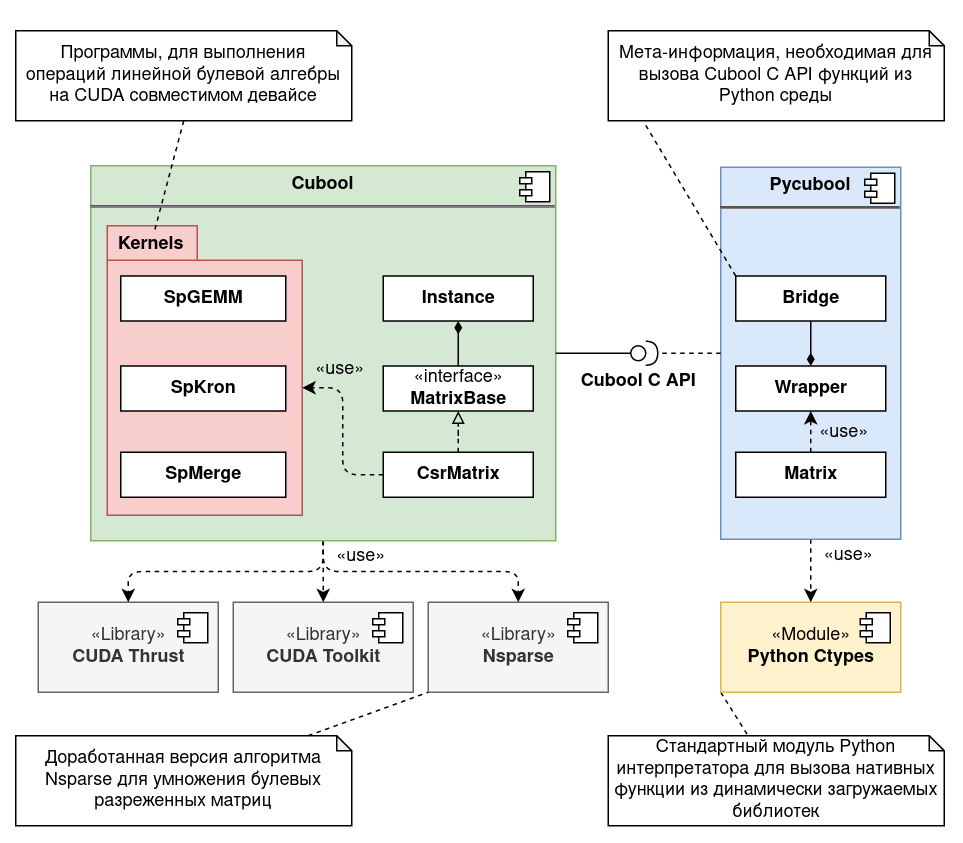
\includegraphics[width=1.0\textwidth]{images/library_architecture.png}
    \caption{Архитектура разработанной библиотеки}
    \label{fig:cubool_architecture}
\end{figure}

\subsubsection{Ядро библиотеки}

Интерфейс библиотеки написан на языке С, что дает возможность использовать данную библиотеку в С компилируемых приложениях или экспортировать ее функции в среды с управляемыми ресурсами через механизмы исполнения внешнего кода. 

Реализация библиотеки представлена классом \textbf{Instance}, который поддерживает глобальное состояние и в момент работы предоставляет контекст выполнения для всех операций библиотеки. Класс \textbf{CsrMatrix} представляет разреженную матрицу булевых значений в формате CSR. Данный класс реализует интерфейс \textbf{MatrixBase} и предоставляет доступ ко всем ранее перечисленным операциям.

Пакет \textbf{Kernels} предоставляет доступ к операциям линейной алгебры, написанным на языке CUDA C++. В качестве основы для реализации операций умножения и сложения матриц использовалась библиотека \textbf{Nsparse}~\cite{inproceedings:cfqp_matrix_with_single_source}, которая была доработана, чтобы добавить возможность динамически конфигурировать механизмы использования видеопамяти. Для реализации произведения Кронекера использовались примитивы библиотеки \textbf{Thrust}, которая позволяет оперировать данными в терминах высокоуровневых операций \textit{свертки}, \textit{отображения} и \textit{префиксной суммы}~\cite{net:cuda_thrust}, которые выполняются на графическом процессоре.     

\subsubsection{Python модуль}

Для работы с примитивами библиотеки на языке Python был разработан модуль \textbf{Pycubool}. Данный инструмент позволит более широкому кругу программистов работать с библиотекой, так как инфраструктура языка Python предоставляет широкий набор утилит для обработки данных, а также поддерживает механизмы автоматического управления ресурсами. Кроме это, использование библиотеки в Python среде позволит переиспользовать существующее решение~\cite{net:cfpq_py_algo} для работы с графовыми данными, которое было получено при реализации алгоритмов~\cite{inbook:kronecker_cfpq_adbis, inproceedings:cfqp_matrix_with_single_source}.

В качестве инструмента для вызова нативных методов, находящихся в скомпилированной библиотеке libcubool.so, используется модуль \textbf{Ctypes}, так как он поставляется вместе с инфраструктурой Python и не требует настройки сторонних зависимостей. 

Класс \textbf{Bridge} хранит мета-информацию о методах и примитивах, импортируемых из нативной библиотеки. Класс \textbf{Wrapper} поддерживает глобальное состояние библиотеки и является точкой входа при импортировании модуля \textbf{Pycubool} в исполняемую среду. Класс \textbf{Matrix} предоставляет операции для работы с разреженными матрицами. 

\subsection{Пример использования}

В качестве примера рассмотрим проблему вычисления \textit{транзитивного замыкания} (англ. transitive closure) для некоторого ориентированного графа без меток $\mathcal{G} = \langle V, E \rangle$. Результатом вычисления транзитивного замыкания является новый в граф $\mathcal{G}_{tc} = \langle V, E_{tc} \rangle$, для которого верно следующее: $e = (v,u) \in E_{tc} \iff \exists v \pi u $ в $\mathcal{G}$. Данную проблему можно решить в терминах линейной алгебры, если представить граф в виде матрицы смежности с булевыми значениями. 

В листинге~\ref{alg:cubool_example} представлен фрагмент кода на языке C, который решает данную задачу. В качестве аргументов функция принимает глобальное состояние библиотеки, матрицу смежности исходного графа, а также указатель на идентификатор, который необходимо использовать при сохранении результирующей матрицы смежности графа после транзитивного замыкания.

В листинге~\ref{alg:pycubool_example} представлен похожий фрагмент кода, однако он уже решает поставленную в задачу на языке Python. Здесь в качестве входного аргумента используется матрица смежности графа, в качестве результата возвращается матрица смежности графа после транзитивного замыкания. Передача состояния библиотеки здесь не требуется, так как он неявно передается во все вызовы нативных методов. 

\definecolor{codegreen}{rgb}{0,0.6,0}
\definecolor{codegray}{rgb}{0.5,0.5,0.5}
\definecolor{codepurple}{rgb}{0.58,0,0.82}
\definecolor{backcolour}{rgb}{1.0,1.0,1.0}

\lstdefinestyle{codelistingstyle}{
    backgroundcolor=\color{backcolour},   
    commentstyle=\color{codegreen},
    keywordstyle=\color{magenta},
    numberstyle=\tiny\color{codegray},
    stringstyle=\color{codepurple},
    basicstyle=\ttfamily\footnotesize,
    breakatwhitespace=false,         
    breaklines=true,                 
    captionpos=b,                    
    keepspaces=true,                 
    numbers=left,                    
    numbersep=5pt,                  
    showspaces=false,                
    showstringspaces=false,
    showtabs=false,                  
    tabsize=2
}

\lstset{style=codelistingstyle}

\begin{algorithm}[h]
\floatname{algorithm}{Listing}
\caption{Пример вычисления транзитивного замыкания с использованием Cubool C API}
\label{alg:cubool_example}
\begin{lstlisting}[language=C++]
CuBoolStatus TransitiveClosure(CuBoolInstance Inst, CuBoolMatrix A, CuBoolMatrix* T) {
    CuBool_Matrix_Duplicate(Inst, A, T);         /** Копируем матрицу смежности А */

    CuBoolSize_t total = 0;
    CuBoolSize_t current;
    CuBool_Matrix_Nvals(Inst, *T, &current);     /** Количество ненулевых значений */

    while (current != total) {                   /** Пока результат меняется  */
        total = current;
        CuBool_MxM(Inst, *T, *T, *T);            /** T += T * T */
        CuBool_Matrix_Nvals(Inst, *T, &current);
    }

    return CUBOOL_STATUS_SUCCESS;
}
\end{lstlisting}
\end{algorithm}

\begin{algorithm}[h]
\floatname{algorithm}{Listing}
\caption{Пример вычисления транзитивного замыкания с использованием Pycubool}
\label{alg:pycubool_example}
\begin{lstlisting}[language=Python]
def transitive_closure(a: pycubool.Matrix):
    t = a.duplicate()                 # Копируем матрицу смежности А
    total = 0                         # Количество ненулевых значений результата

    while total != t.nvals:           # Пока результат меняется
        total = t.nvals
        pycubool.mxm(t, t, t)         # t += t * t

    return t
\end{lstlisting}
\end{algorithm}